\documentclass[french,a4paper]{article}
\setcounter{tocdepth}{4}
\setcounter{secnumdepth}{4}
\usepackage{float}
\usepackage{graphicx}
\usepackage{hyperref}
\usepackage{pdfpages}
\newcommand{\tabitem}{\textbullet~~}
\newcommand{\HRule}{\rule{\linewidth}{0.5mm}}
\usepackage{multirow}
\graphicspath{{img/}}
\title{PPII}
\usepackage[bottom=2.5cm,top=2.5cm,left=2.5cm,right=2.5cm]{geometry}
\author{Noé Steiner - Alexis Marcel - Lucas Laurent - Mathias Aurand-Augier}
\date{Janvier 2023}
\begin{document}

%\maketitle

\begin{titlepage}
    \begin{center}

    
\includegraphics[width=0.5\textwidth]{tele_univ.png}

    \textsc{\Large Rapport final de Projet Pluridisciplinaire d'Informatique Intégrative}\\[1.5cm]

    \HRule \\[0.4cm]
    { \huge \bfseries Les jardins partagés\\[0.4cm] }

    \HRule \\[2cm]

    \begin{minipage}{0.4\textwidth}
      \begin{flushleft} \large
        Alexis MARCEL\\
        Lucas LAURENT\\
        Noé STEINER\\
        Mathias AURAND-AUGIER\\
      \end{flushleft}
    \end{minipage}
    \begin{minipage}{0.4\textwidth}
      \begin{flushright} \large
        \emph{Responsable du module :}\\
        Olivier FESTOR\\
        Anne-Claire HEURTEL\\
        Gerald OSTER\\
      \end{flushright}
    \end{minipage}

    \vfill

    {\large 6 Janvier 2023}

  \end{center}
\end{titlepage}
\newpage
\tableofcontents
\newpage
\section{Base de donnée}
\subsection{Conception}
\subsubsection{Que faut-il dans notre base ?}
Pour la base de donnée, nous aurons besoin de stocker plusieurs informations. Nous aurons besoin en premier lieu de stocker 
toutes les données concernant l'utilisateur (les informations de son compte à savoir son identifiant ou son mot de passe par ex), nous
aurons également de stocker des données concernant les jardins que les utilisateurs vont créer (comme l'endroit où il se trouve par exemple, 
le nombre de personne qui en font partie). Lorsque les jardins seront crées, nous aurons besoin de caractériser les parcelles de jardin 
(les légumes qu'on y cultive ou encore l'état dans lequel elle est : a t'elle été labouré). Afin d'avoir une vue d'ensemble sur les 
différentes missions au sein des jardins, nous aurons également besoin de caracteriser les differentes tâches à faire (date limite,
la personne qui s'en occupera...). 
\subsubsection{Schéma entité-association}

Maintenant que nous savons ce que nous aurons à stocker, nous ponvons commencer la réalisation de notre schéma entité-asociation
en respectant les contraintes logiques de cardinalités suivantes : 
\begin{itemize}
    \item Une personnes peut posséder un ou plusieurs jardins mais un jardin ne peut avoir qu'un propriétaire
    \item Un jardin peut avoir plusieurs parcelles mais une parcelle est completement associé à son jardin.
    \item Une personne peut faire autant de tache qu'elle veut, et de même, plusieurs personnes peuvent participer à une même tache.
\end{itemize}
Ainsi, on obtient le schéma suivant : 

\begin{figure}[H]
    \centering
    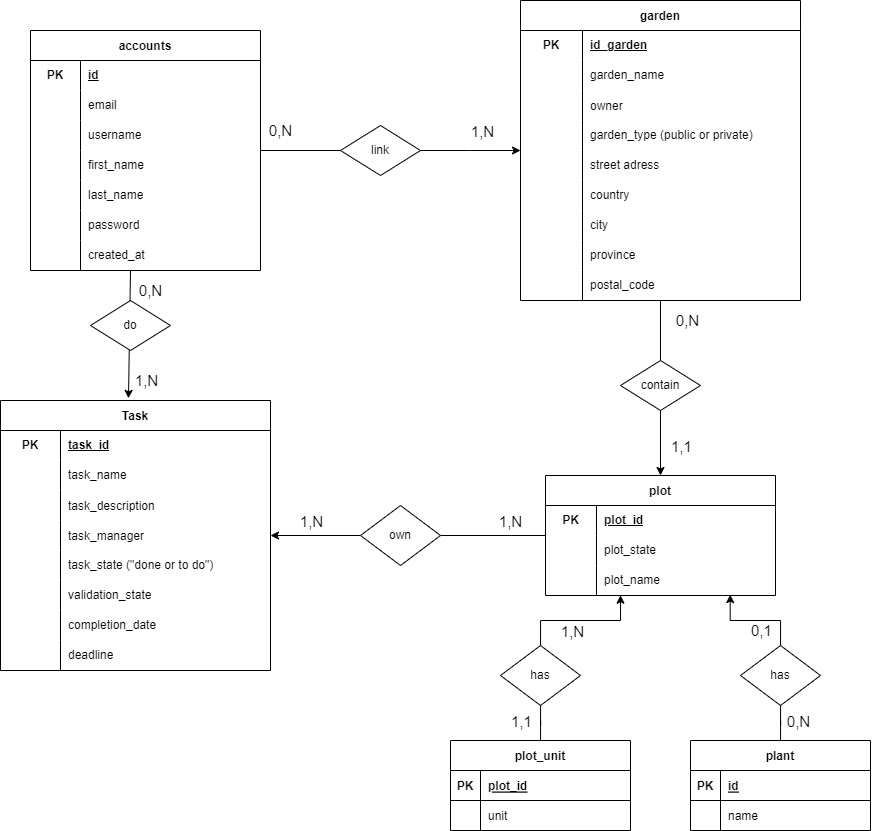
\includegraphics[width=1\textwidth]{img/Schema_entite_association_PPIIversion2.drawio.png}
    \caption{Schéma entité-association}
\end{figure}

\subsubsection{Mise en 3ème forme normale}
Pour finaliser la conception de notre base, il faut maintenant transformer les entités et associations décrites dans le schéma en 
relation, que nous mettrons ensuite sous troisieme forme normale : on obtient ainsi les relations suivantes : 
\begin{itemize}
    \item account(id, email, username, first name, last name, password, created at)
    \item garden(garden id, owner, garden name, manager, garden type, street adress, country, city, province, postal code)
    \item plot(plot id, garden id, plot state, plot name, cultivated vegetables)
    \item task(task id, plot id, task name, task description, task manager, task state, completion state, validation state, deadline)
    \item plot unit(plot id, unit)
    \item do(account id, task id)
    \item link(account id, garden id)
\end{itemize}
\subsection{Implémentation}
\subsubsection{SQL alchemy}
SQLAlchemy est un ORM (Object-Relational Mapping) permettant de manipuler la base de données via des objets python. Les requêtes en 
python sont ainsi "traduites" en SQL et la réponse reçu se présentera sous la forme d’un objet python avec lequel on peut interagir.
SQLAlchemy constitue donc un pont entre la base de données et notre application. Pour que l’ORM puisse savoir où se situe notre 
base de données (pour pouvoir l’interroger), on doit définir des modèles. 
On doit ainsi lier les éléments de notre table avec des classes python dans lesquels on indiquera le type de chaque champ. 
Les sessions de SQLAlchemy permettent de gérer les transactions SQL, autrement dit un ensemble de requêtes. Si l'une d'elles échoue,
l'ensemble de la transaction est annulée et aucune requête n'est communiquée à la base. L’avantage de ce système est la sécurité. 
Par exemple, si on crée un utilisateur et que le requête permettant la création des propriété de l’utilisateur dans une autre table 
(mot de passe) échoue,l’ensemble des requêtes est alors annulé et la base est corrompu par un utilisateur sans permission.

\subsubsection{Création de la base}
En utilisant le systeme de gestion de base de données sqlite, nous avons crée notre base dans un fichier data.db avec le script 
sauvegarder dans un fichier nommée "creation table.sql". Ces deux fichiers sont dans le dossier Data situé à la racine du Backend.  

Dans le dossier models, situé à la racine du backend, nous avons crée les modèles, les classes python associé aux élements de la base. 
La connection à la base de donnée via SQLAlchemy est codé dans fichier intitulé bdd.py

\newpage
\section{Implémentation Partie Web}
\subsection{structure de l'application}
Nous avons choisi de séparer la partie affichage coté utilisateur (Frontend) et la partie gestion de l'application coté serveur (Backend).
Les deux communiquent ensembles via une API. 
Dans le backend, se trouvent les differentes fonctionnalités se déroulant coté serveur tel que : l'authentification ou encore la gestion 
de la base de données. Le backend est un serveur flask(et les fonctions sont donc codés en python)
Dans le front end, on utilise une librairie Javascript appelé React.

\subsection{Fonctionnalités de l'application}
\subsubsection{Authentification}
Pour accèder aux fonctionnalités de l'application, une insciption est nécessaire. Nous avons ainsi besoin de creer une Authentification.
L'utilisateur doit d'abord se créer un compte. Par la suite, si l'utilisateur veut se connecter, il devra rentrer les informations données lors de 
son inscription. 

Nous avons ainsi séparé l'Authentification en plusieurs parties : les trois premieres situé dans le fichier Authentification.py situé
la dossier Route (racine backend) et la dernieres dans le fichier auth.py situé dans middlewares.
\begin{itemize}
    \item La fonction signup (inscription) récupère dans un permier temps les données rentrées par l'utilisateur. Ensuite, la fonction
verifie si l'email est déjà enregister. Si il l'est alors l'utilisateur ne peut pas s'inscire. Sinon, la fonction hache le mot de 
passe (elle le crypte), avant de crée un nouveau compte. Pour finir, la fonction renvoie une réponse avec un cookie (jeton JWT).
    \item La fonction signin (connexion) récupère l'e-mail et le mot de passe d'un utilisateur, vérifie si l'utilisateur existe et si 
le mot de passe est correct, et si c'est le cas, il renvoie un cookie avec un jeton JWT.
    \item La fonction signout (déconnexion) déconnecte l'utilisateur en supprimant le cookies.
    \item La fonction authtest utilise la fonction authentificate se trouvant dans le fichier auth.py du dossier middlewares. Cette 
fonction récupère d'abord le token se trouvant dans le cookies (envoyé par la fonction signin ou signup), et verifie si le token existe
avant de donner l'accès à l'application.
\end{itemize}

\subsubsection{Gestion de compte et présentation des jardins}
Dans le backend, la gestion du profil est dans le fichier appelé profile.py. Cette gestion se décompose en plusieurs fonctions :
\begin{itemize}
    \item La fonction get information récupère les informations de la base de données et les renvoie sous la forme d'un objet json, 
la récupération de la photo de profil se fait via la fonction get image, qui va chercher la photo dans le dossier static du backend.
    \item La fonction modify profile permet à l'utilisateur de modifier son profil. Cette fonction récupère d'abord le tuple de la base 
associé à l'utilisateur en vue de le modifier. La fonction récupère ensuite les informations tapés par l'utilisateur à condition qu'elles 
existent, le tuple est ainsi modifié avec les nouvelles informations avant d'être réinjecté dans la base.
\end{itemize}
\subsubsection{Gestion des jardins : creation, destruction, modification, management}
Dans le backend, la gestion des jardins s'étend sur 2 fichiers. Au sein du fichier garden.py se trouve les fonctionnalités suivantes : 
\begin{itemize}
    \item La fonction get all garden : permet de montrer à l'utilisateur les jardins qu'il possède. Elle récupère les jardins associés
à l'id de l'utilisateur (en effectuant une jointure entre 2 tables), elle utilise ensuite une fonction (issue du dossier lib, fichier
garden.helper) qui va renvoyer les informations concernant chaque jardin sous la forme d'objet json. 
    \item La fonction create permet de créer un jardin. Elle récupère dans un premier temps toutes les informations rentrés par 
l'utilisateur sur son jardin (photo, nom...). Les informations sont ensuite mise dans la base et la photo dans le dossier Static.
    \item La fonction 

\end{itemize} 
\subsection{}
\subsubsection{}
\subsubsection{}
\subsubsection{}
\subsection{Test et performance}
\subsubsection{}
\subsubsection{}
\subsubsection{}

\newpage
\section{Algorithme}
\subsection{Principe de l'algorithme}
\subsection{Implémentation}
\subsection{Analyse en complexité}
\subsection{Test de validité de l'algorithme}
\subsection{Analyse de performance}

\newpage
\section{Gestion de projet}
\subsection{Équipe de projet}
Ce projet est un projet local réalisé en groupe de 4 personnes~:
\begin{itemize}
    \item Alexis MARCEL
    \item Lucas LAURENT
    \item Noé STEINER
    \item Mathias AURAND-AUGIER
\end{itemize}
Le comité de pilotage est constitué de~:
\begin{itemize}
    \item Anne-Claire HEURTEL
    \item Olivier FESTOR
    \item Gérald OSTER
\end{itemize}
Ces personnes constituent les parties prenantes de notre projet ainsi que les acteurs influents sur le livrables.
\begin{figure}[H]
    \centering
    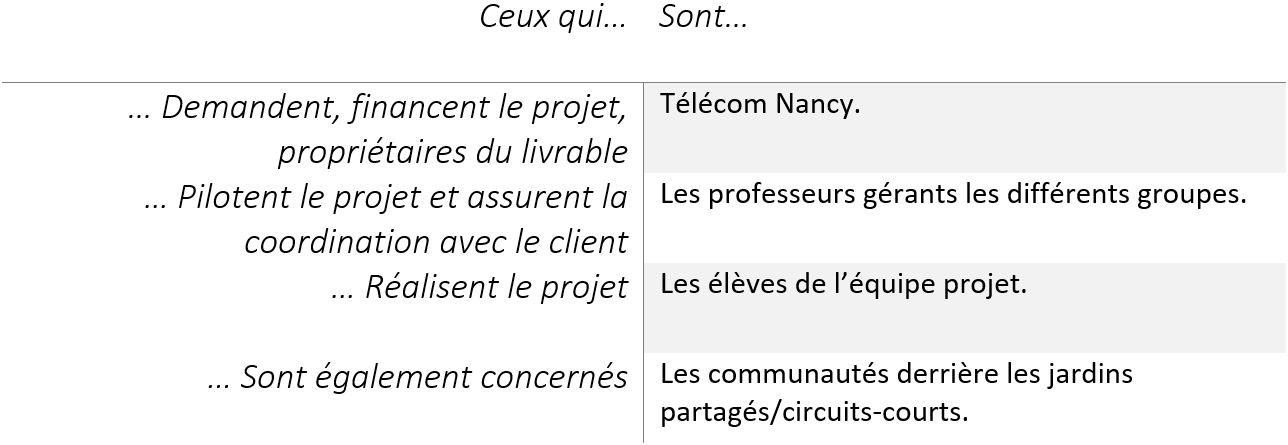
\includegraphics[width=0.75\textwidth]{img/parties_prenantes.png}
    \caption{Parties prenantes}
\end{figure} 
\subsection{Organisation au sein de l’équipe projet}
Nous avons réalisé plusieurs réunions, en présentiel dans les locaux de Télécom Nancy mais également sur en visio-conférence sur Discord. Ces réunions nous ont permis de mettre en commun nos avancés régulièrement, de partager nos connaissances sur des problématiques et de nous organiser de manière optimale.
Les comptes rendus des réunions réalisés sont présents dans l’\hyperlink{annexe1}{Annexe 1}.

De plus, dès le début de notre projet nous avons mis en place un projet Trello. Trello est une application permettant d’organiser facilement un projet en reposant sur une organisation en planches listant des cartes, chacune représentant des tâches. Ces tâches peuvent ensuite être déplacées permettant de découper notre projet en plusieurs jalons dynamiquement.
\begin{figure}[H]
    \centering
    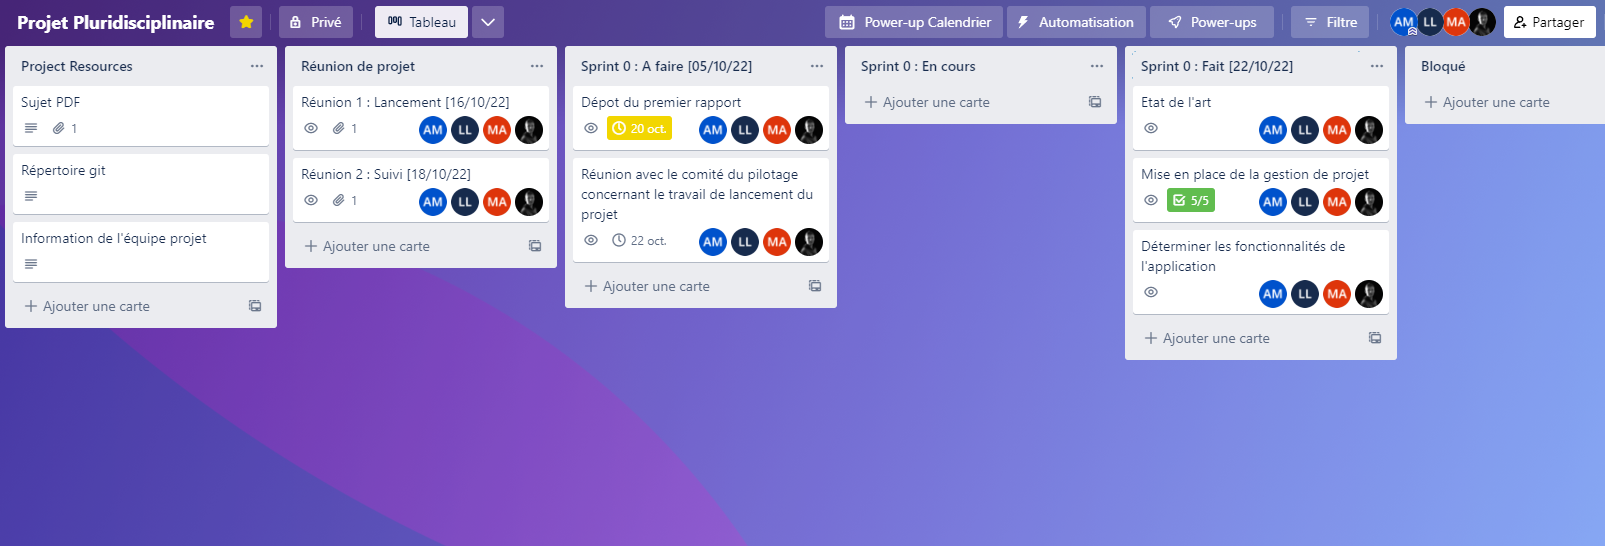
\includegraphics[width=0.75\textwidth]{img/trello.png}
    \caption{Organisation Trello}
\end{figure} 

Ensuite, nous avons utilisé GitLab pour gérer les différentes versions du développement de notre application, ainsi que les différentes branches nous permettant de travailler simultanément sans conflit.

Enfin, la rédaction des differents comptes rendu de réunion et des rapports ont été rédigé en \LaTeX.

\subsection{Objectifs SMART}
La méthode SMART que l'on rappelle ci-dessous nous a permis de définir nos différents objectifs :

\begin{figure}[H]
    \centering
    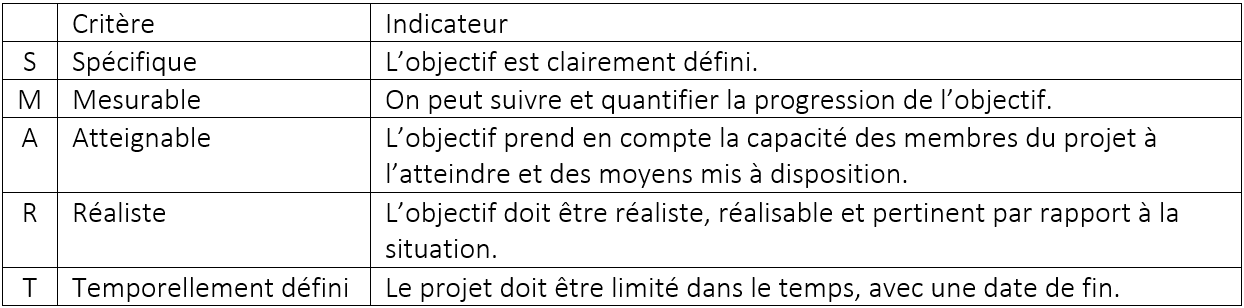
\includegraphics[width=1\textwidth]{img/SMART.png}
    \caption{Objectif SMART}
\end{figure}

\subsection{Matrice des objectifs}
Nous avons conçu, à l'aide de la méthode SMART, la matrice des objectifs suivante :

\begin{figure}[H]
    \centering
    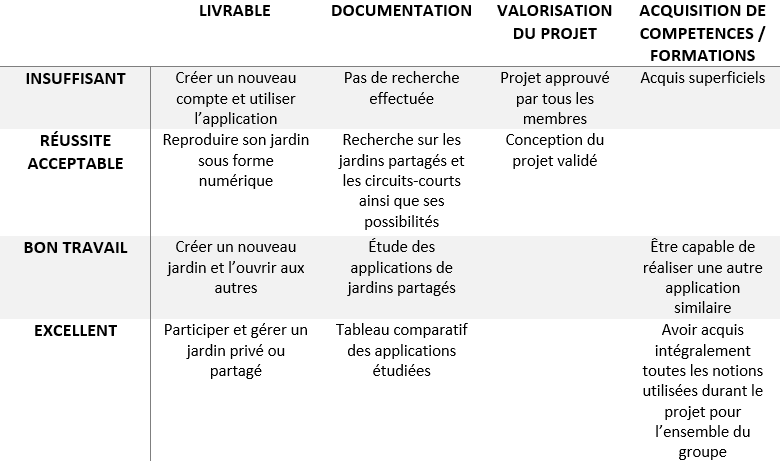
\includegraphics[width=1\textwidth]{img/matrice_des_objectifs.png}
    \caption{Matrice des objectifs}
\end{figure}

\subsection{Triangle qualité-cout-délai}
Afin d’établir des objectifs cohérents, et réalisables dans les délais, nous avons réalisé le triangle qualité-coût-délai. On remarque ainsi, les délais étant courts, que nous avons tout intérêt à ne pas se fixer des objectifs trop ambitieux sous peine de devoir renoncer à certaines fonctionnalités et de ne pas rendre le livrable annoncé initialement.

\begin{figure}[H]
    \centering
    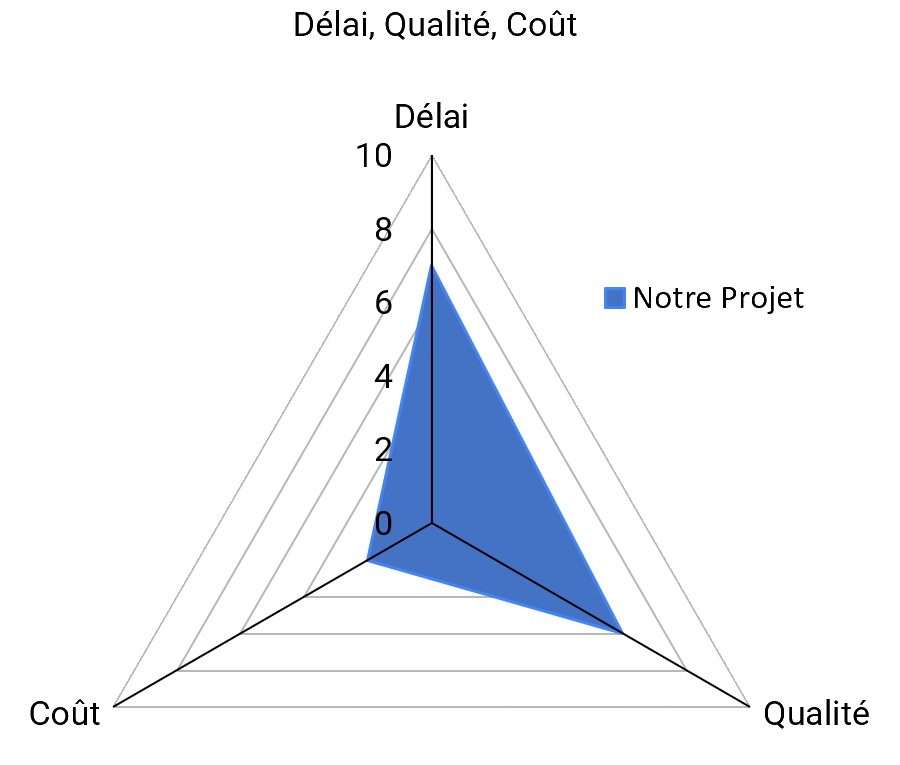
\includegraphics[width=0.5\textwidth]{img/triangle_QCD.png}
    \caption{Triangle DQC}
\end{figure}

\subsection{Matrice SWOT}
Afin d’avoir une vision plus globale de nos ressources et des facteurs interne et externe agissant sur le projet, nous avons ensuite réalisé la matrice SWOT (Strengths, Weaknesses, Opportunities, Threats) de notre projet.

\begin{figure}[H]
    \centering
    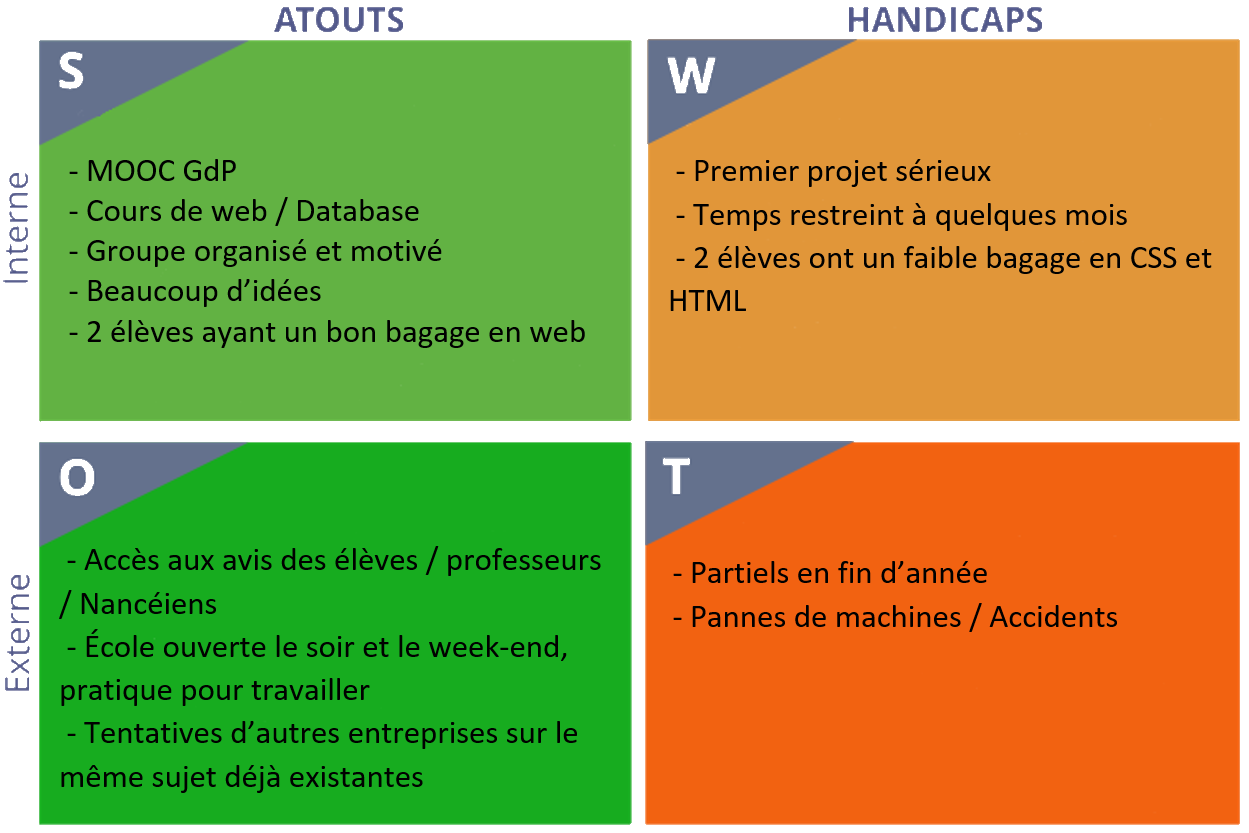
\includegraphics[width=0.75\textwidth]{img/SWOT.png}
    \caption{Matrice SWOT}
\end{figure} 

On peut ainsi remarquer que notre projet présente de nombreux points fort notamment grâce aux connaissances acquises lors des cours de Télécom Nancy mais également de part l’expérience forte de deux des membres de l’équipe projet qui ont déjà réalisé des applications similaires.  Cependant, plusieurs facteurs internes constituent nos faiblesses notamment les courts délais qui nous oblige à être concis et efficaces dans notre travail, ou encore le faible bagage informatique de deux des membres de l’équipe. Néanmoins, ces lacunes constituent pour eux l’opportunité d’apprendre, et de progresser avec l’aide des membres expérimentés de l’équipe.

De plus, nous devons anticiper les charges de travail dans le cadre de notre formation à Télécom Nancy qui s'avèrent être plus élevée en décembre lors des partiels de fin d'année. Nous allons donc devoir prendre cela en compte dans notre gestion des tâches. 

\subsection{Profil de projet}
Afin d’avoir une vision plus globale sur notre projet, nous avons également réalisé le profil du projet (le budget étant égal à 0, nous avons choisi de ne pas le représenter dans notre profil). On remarque que, du fait des nombreuses fonctionnalités que nous avons l’intention d’implémenter dans notre application, que notre projet est de taille moyenne mais de complexité élevée.

Cependant, les enjeux du projet ne sont pas très importants (en dehors de la note finale qui compte dans notre moyenne) car l'échec du projet n'engendra pas la chute d'une organisation et le budget est négligeable.

De plus, au vu de l’état de l’art établi, l’innovation du projet est importante puisque nous avons choisi de combiner différentes fonctionnalités existantes de plusieurs applications et d’en rajouter de nouvelles.

\begin{figure}[H]
    \centering
    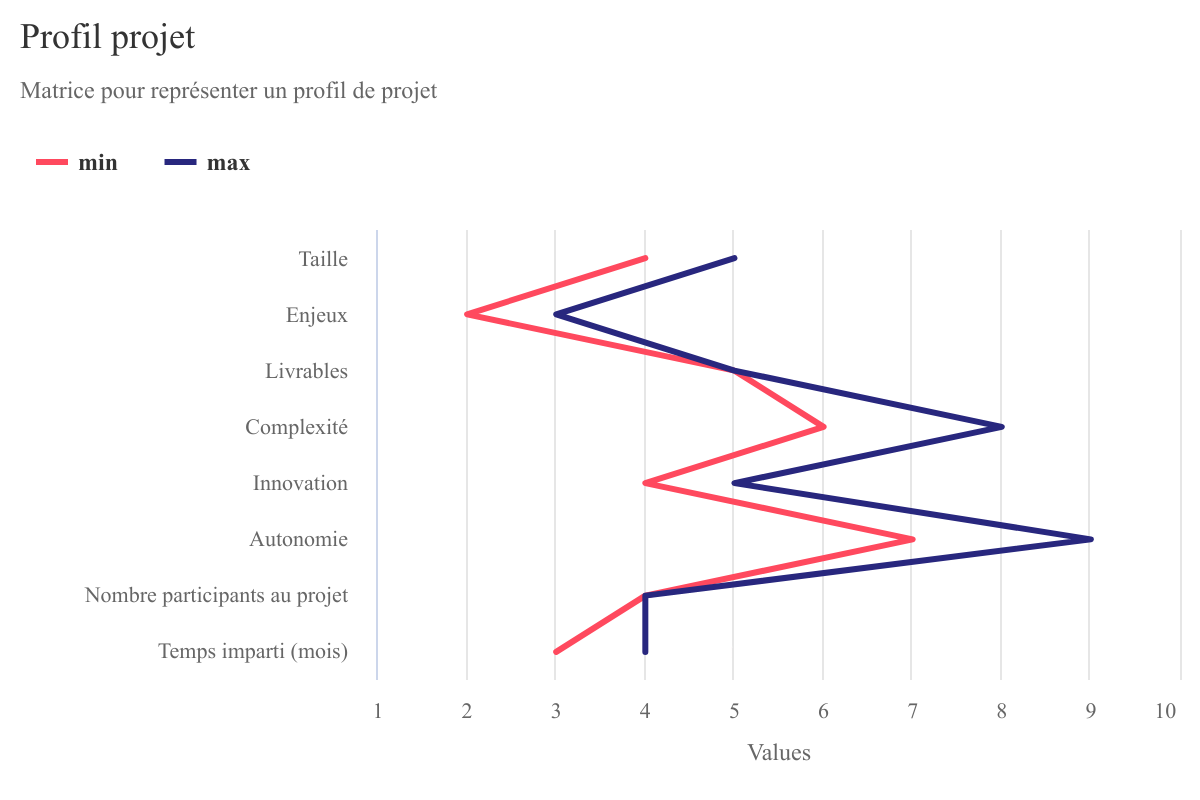
\includegraphics[width=0.75\textwidth]{img/profil_projet.png}
    \caption{Profil du projet}
\end{figure} 

\subsection{WBS~: comment concrétiser l’application}
Ceci étant fait, nous avons maintenant choisi de détailler les lots de travail à effectuer pour fabriquer notre application. Nous avons ainsi réalisé le WBS (Work Breakdown Structure) de notre application~: il apparait ainsi les grandes étapes de notre projet que sont~: definition du cadre de l’application, développement des fonctionnalités de l’application et écriture du rapport.
\begin{figure}[H]
    \centering
    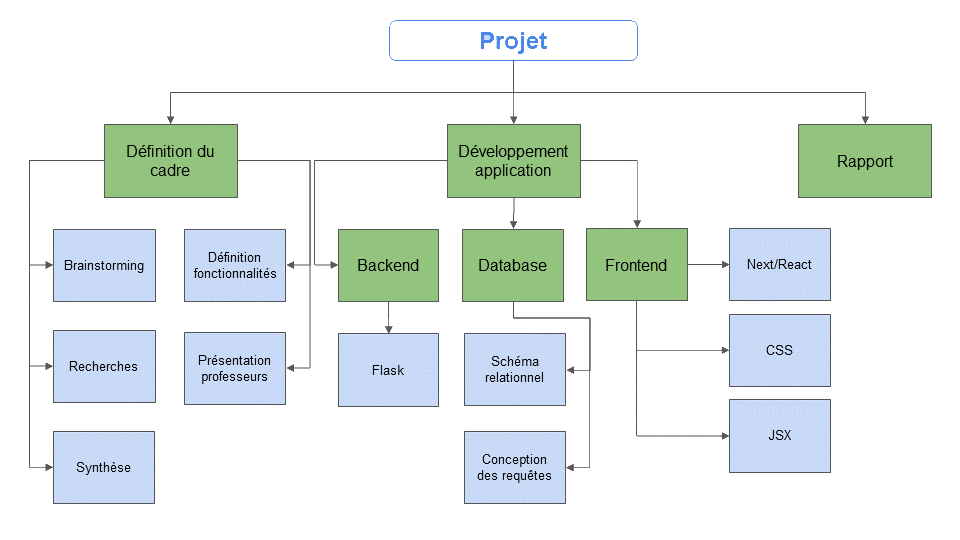
\includegraphics[width=0.75\textwidth]{img/WBS.png}
    \caption{WBS}
\end{figure} 

\subsection{Diagramme de Gantt~: planification}
Maintenant que nous avons un détail des lots de travail qui constitue notre application, il faut maintenant les mettre en relation pour créer un planning efficace où chaque tâche est effectuée dans l’ordre.
\begin{figure}[H]
    \centering
    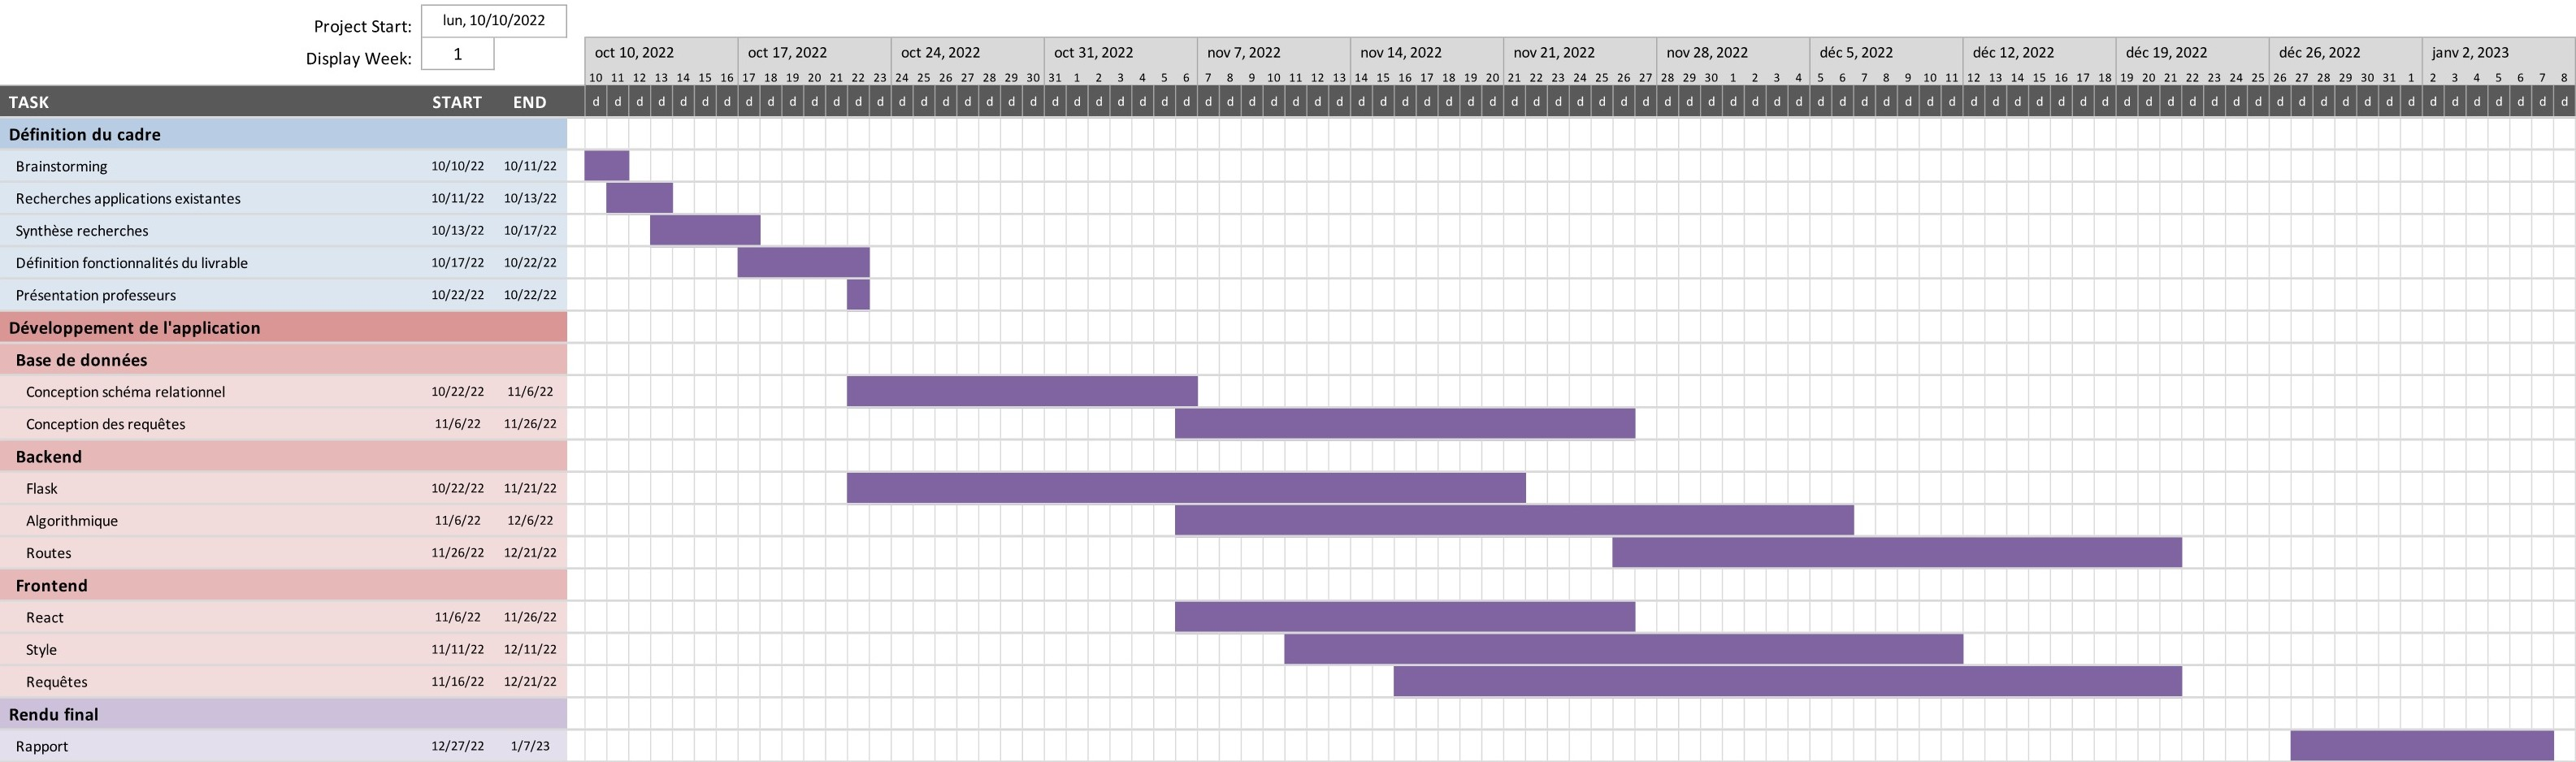
\includegraphics[width=1\textwidth]{img/gantt.png}
    \caption{Diagramme de GANTT}
\end{figure} 
Ce diagramme est une première version générale des tâches à effectuer, il sera modifié et détaillé davantage une fois la conception et les maquettes du projet réalisé.

\subsection{Matrice RACI}
Maintenant que toutes les étapes sont planifiées, nous devons répartir le travail entre les membres de l’équipe. On utilise ainsi une matrice RACI synthétisant les rôles de chacun.

\begin{figure}[H]
    \centering
    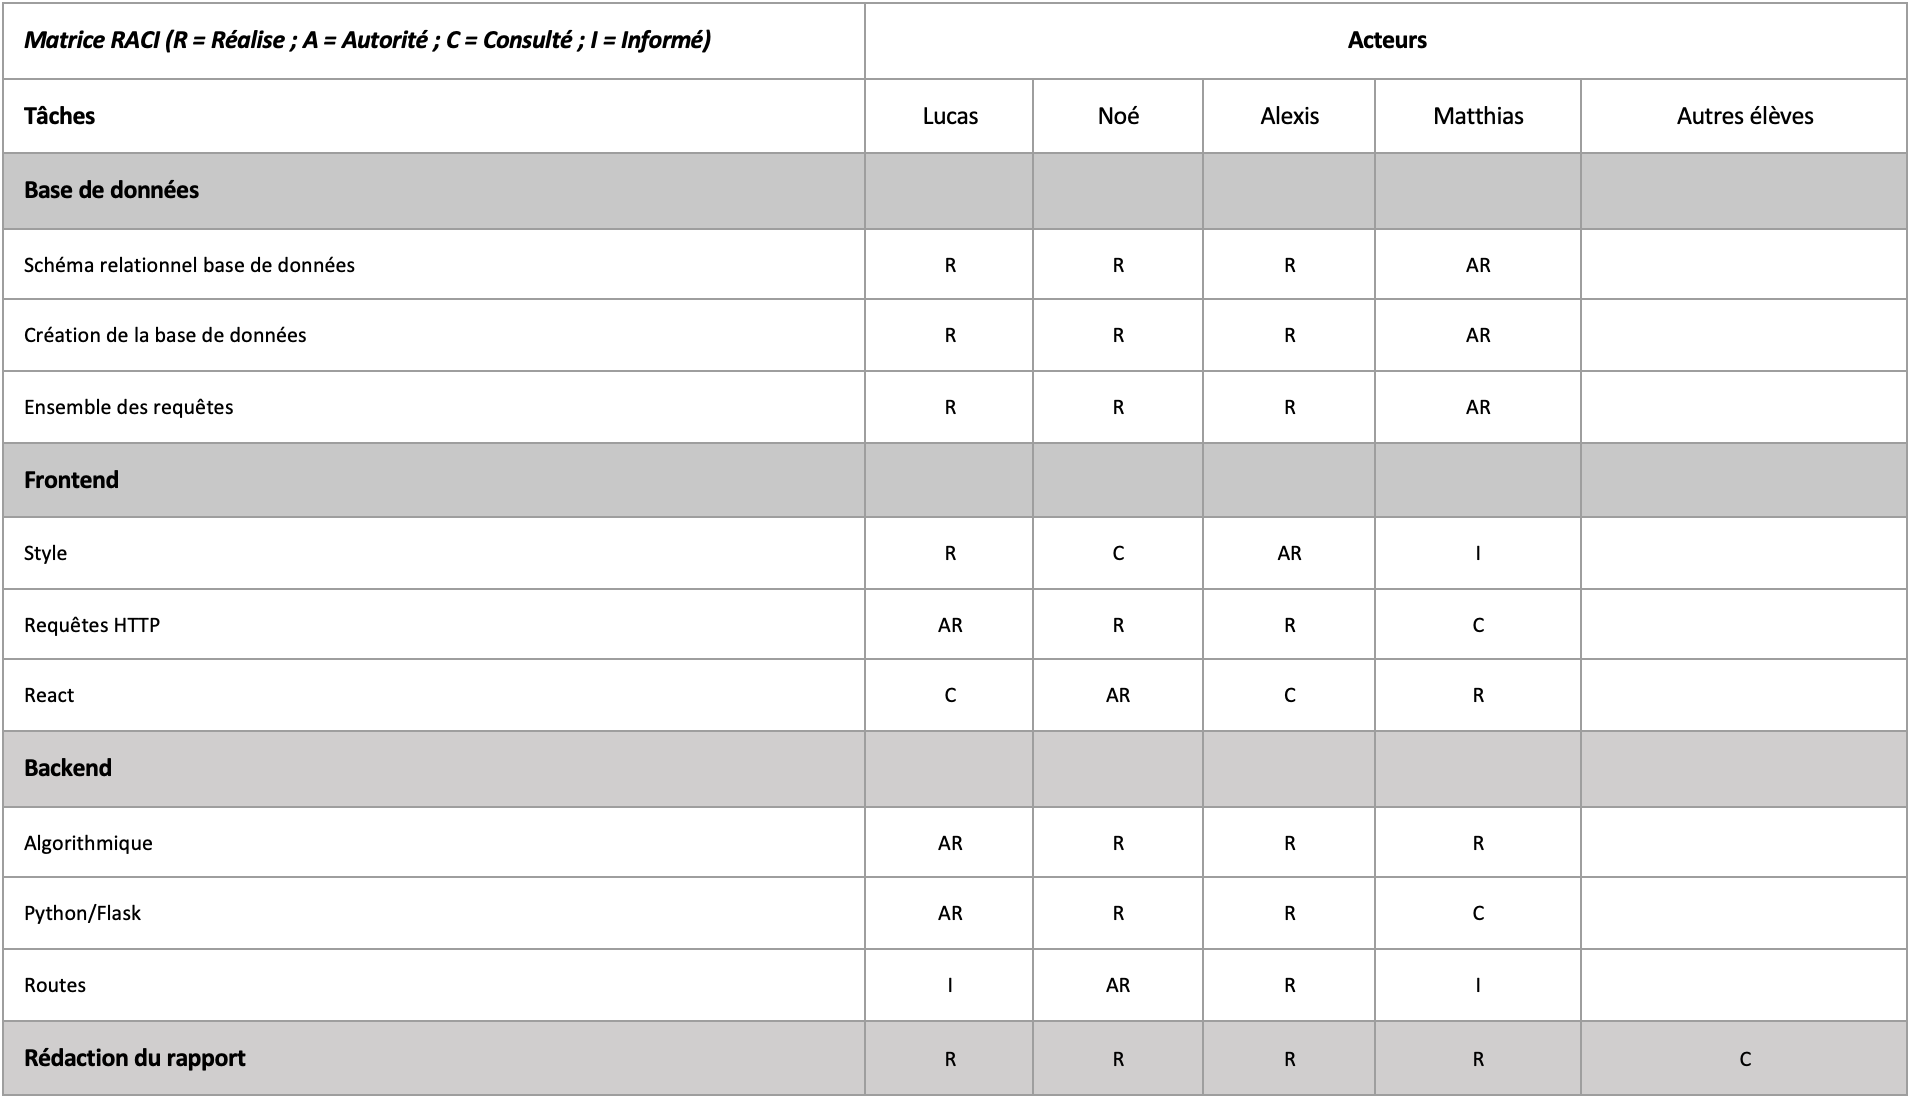
\includegraphics[width=1\textwidth]{img/RACI.png}
    \caption{Matrice RACI}
\end{figure} 

\subsection{Gestion des risques}
Nous avons également penser à prévoir une partie des risques pouvant se dresser sur notre route, les risques les plus classiques étant 
la gestion du temps et le manque de comprehension de certaines personnes de l'équipe
\begin{figure}[H]
    \centering
    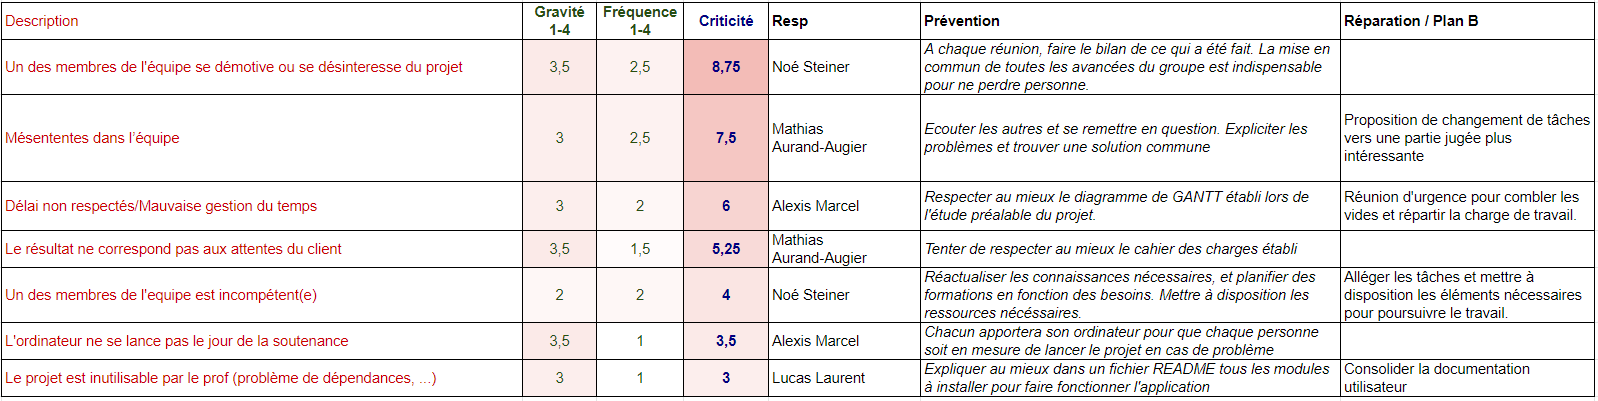
\includegraphics[width=1\textwidth]{img/Plan_gestion_risque.png}
    \caption{Plan de gestion des risques}
\end{figure} 

\section{Conclusion}

\section{Annexes}
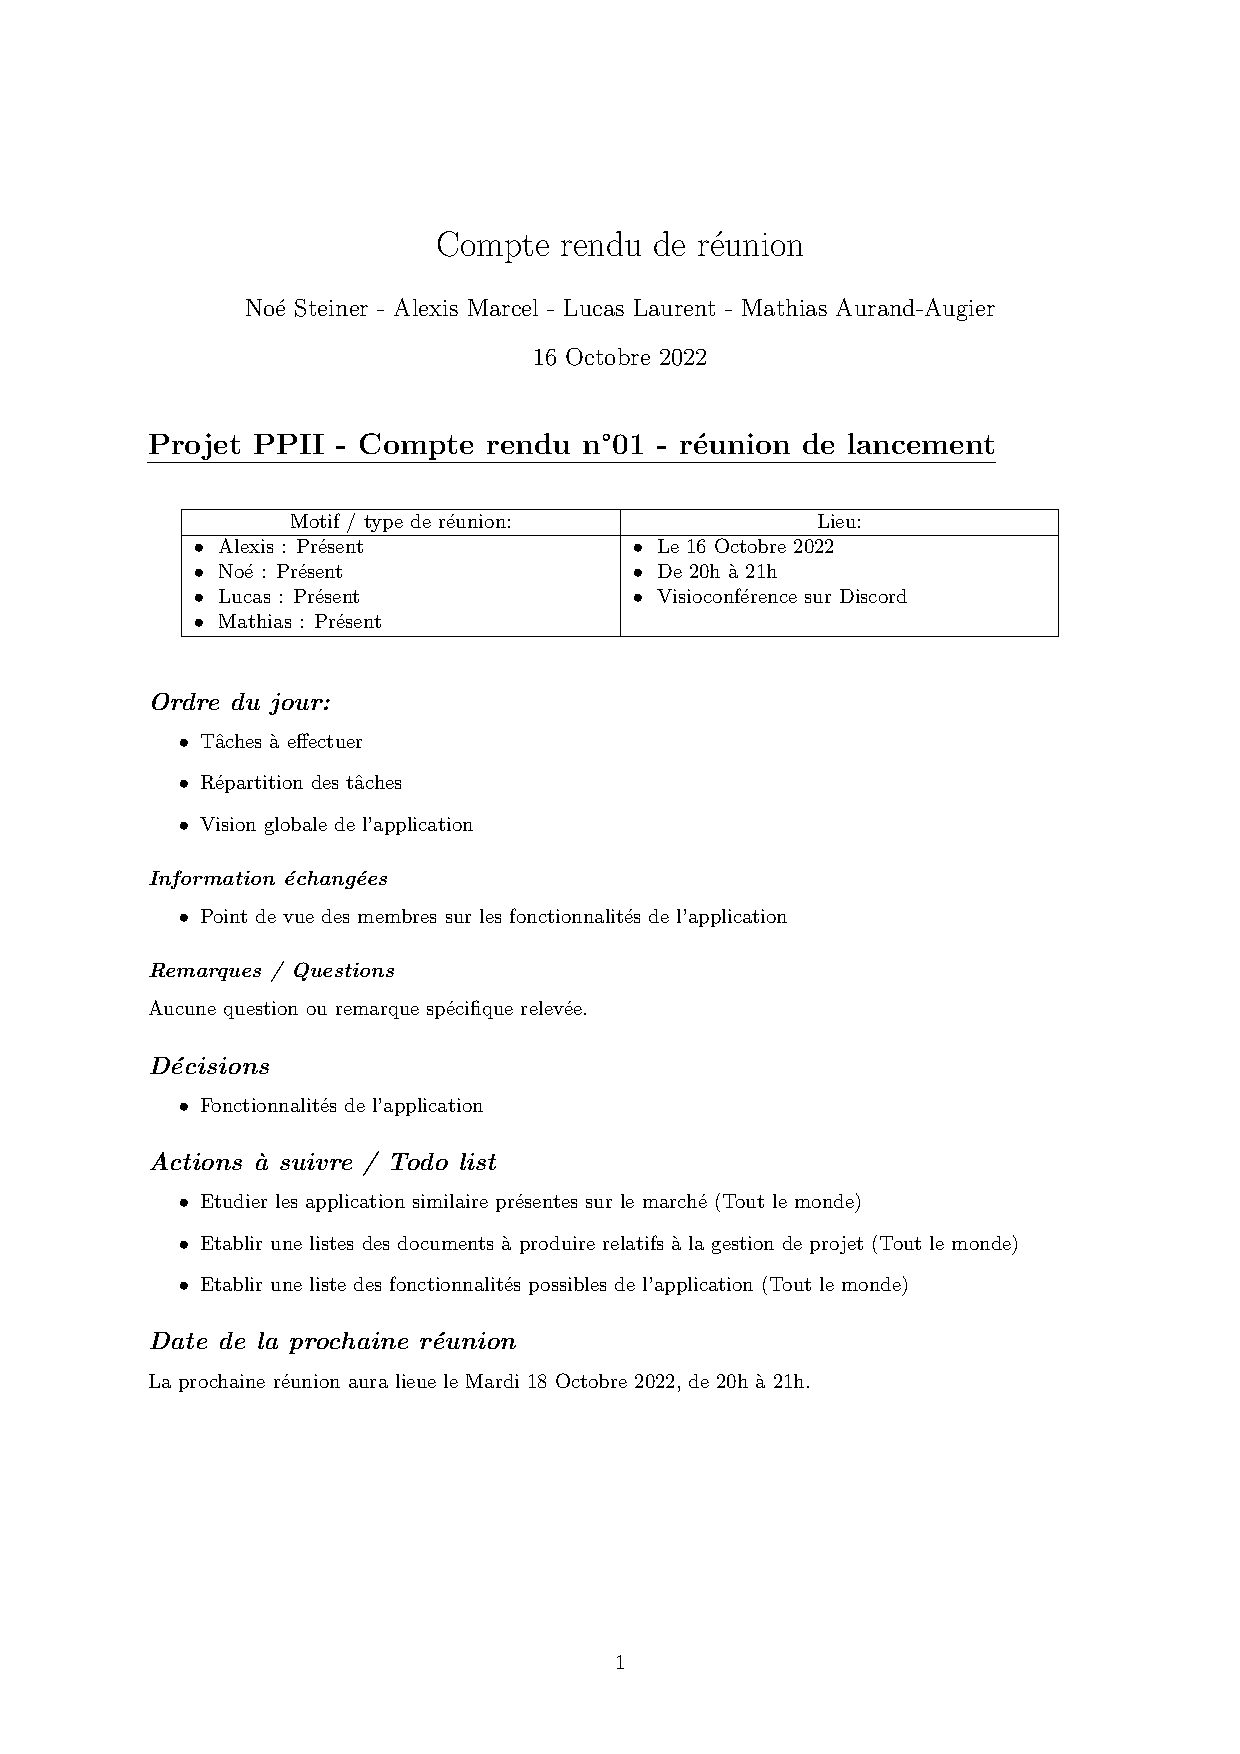
\includepdf[pages=1]{../../cr_reu/octobre/16/cr_16_octobre.pdf}
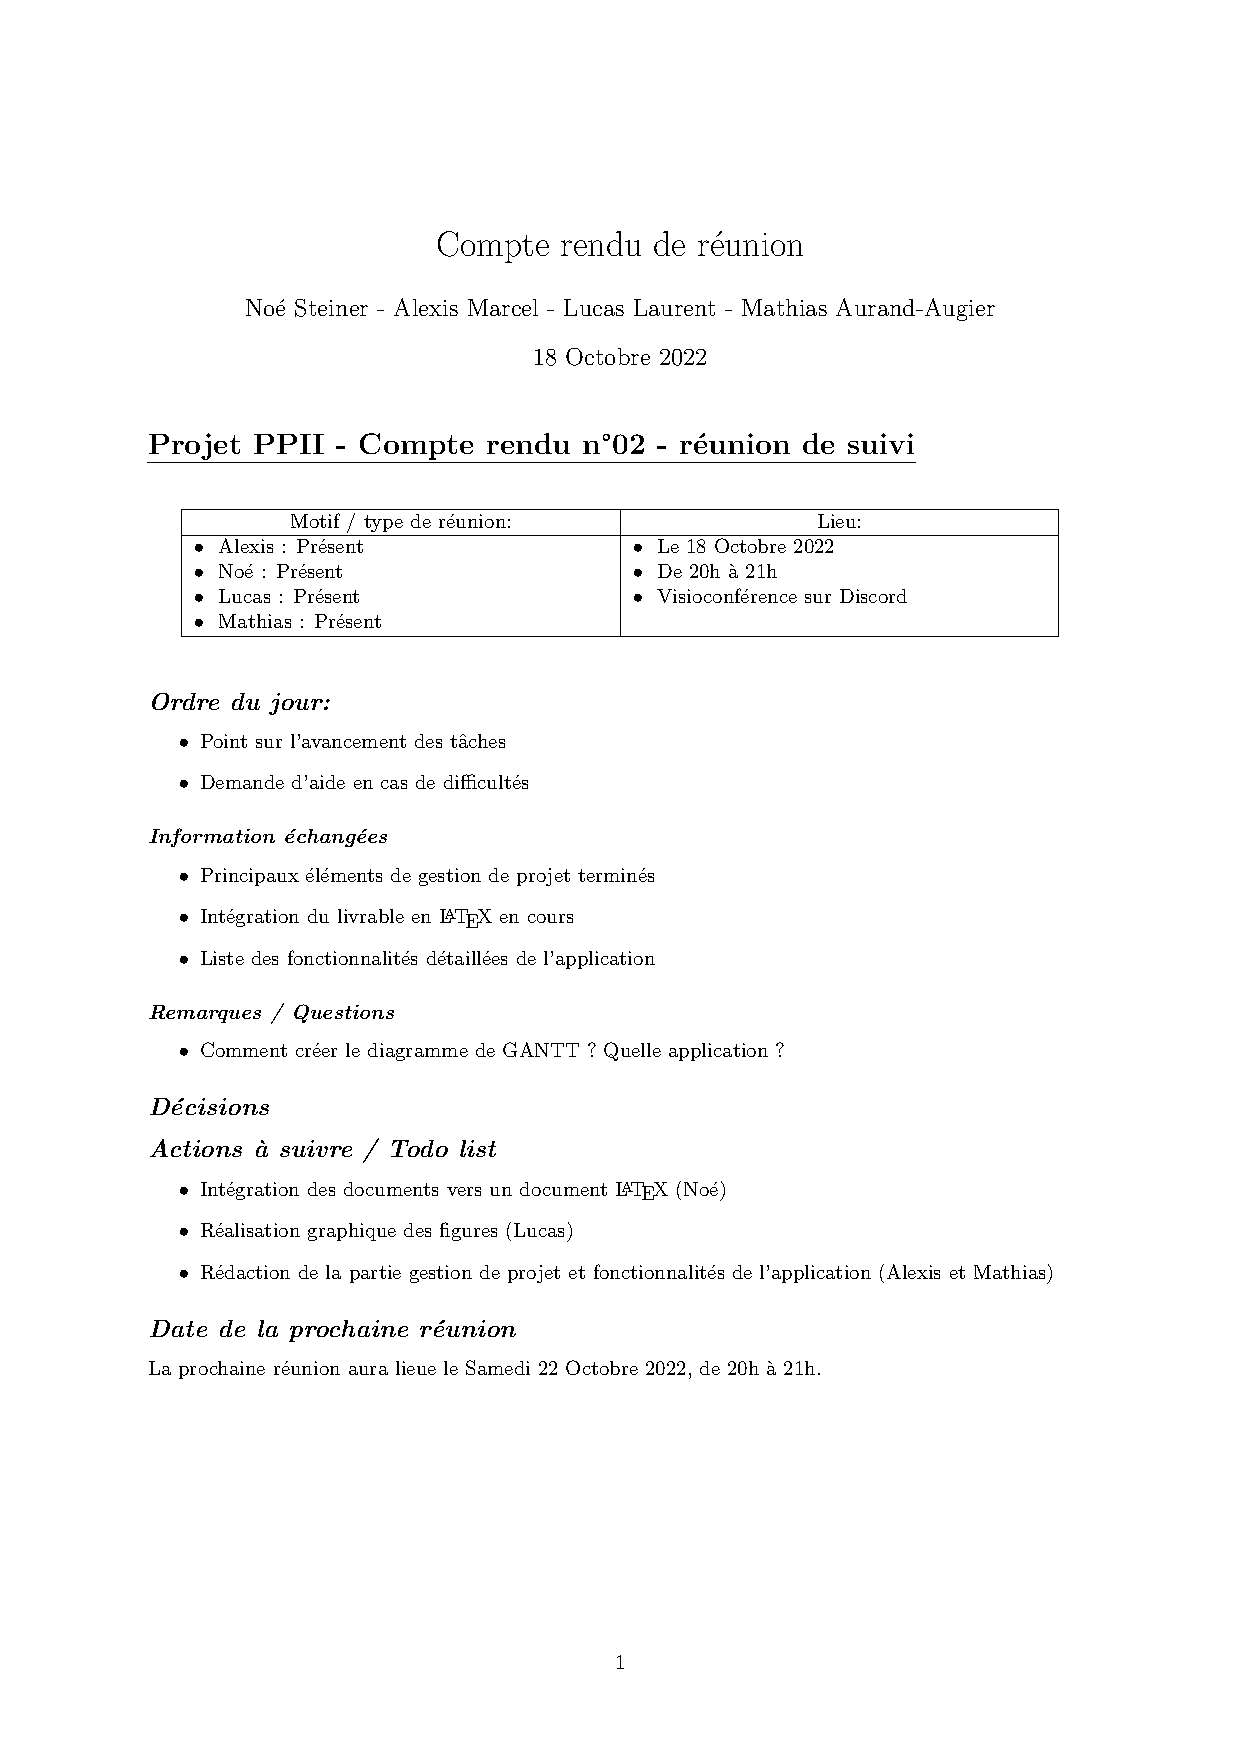
\includepdf[pages=1]{../../cr_reu/octobre/18/cr_18_octobre.pdf}
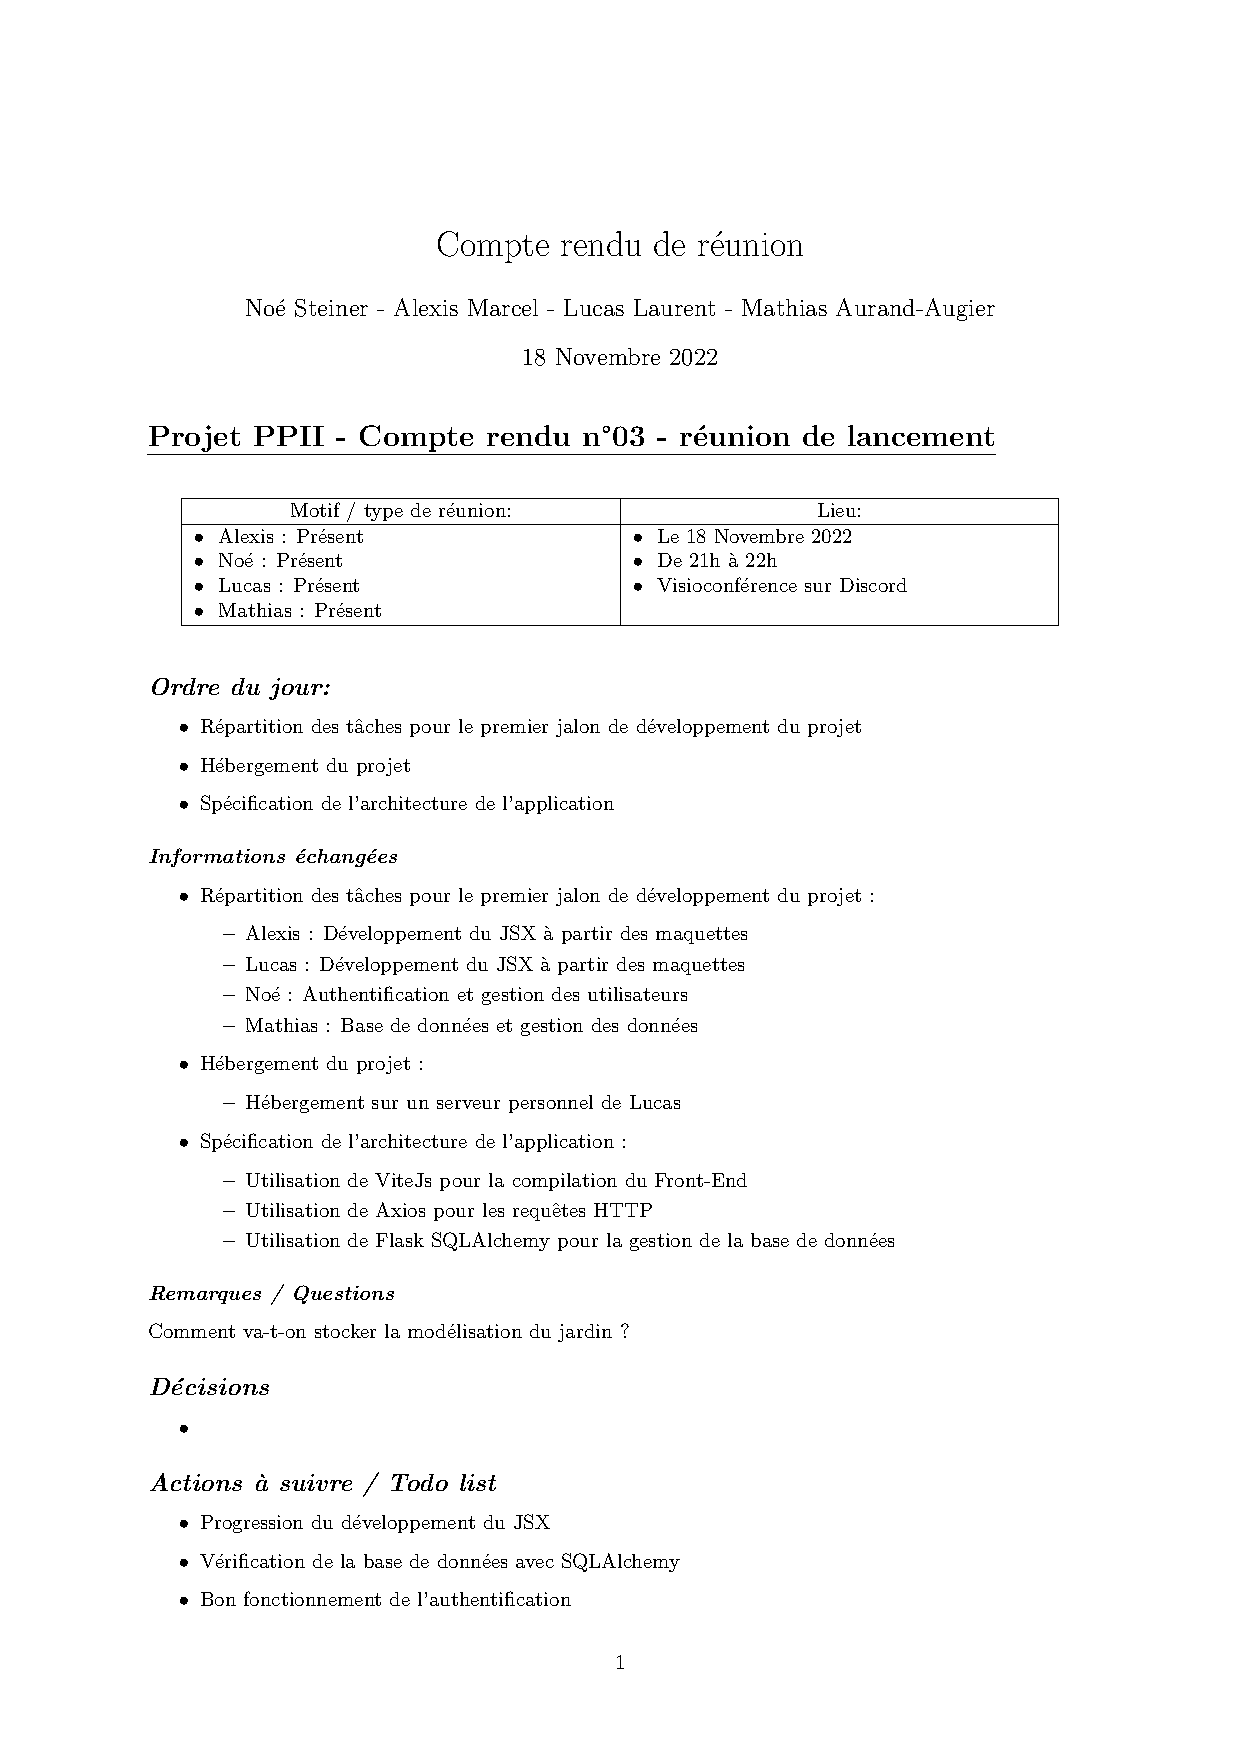
\includepdf[pages=1]{../../cr_reu/novembre/18/cr_18_novembre.pdf}
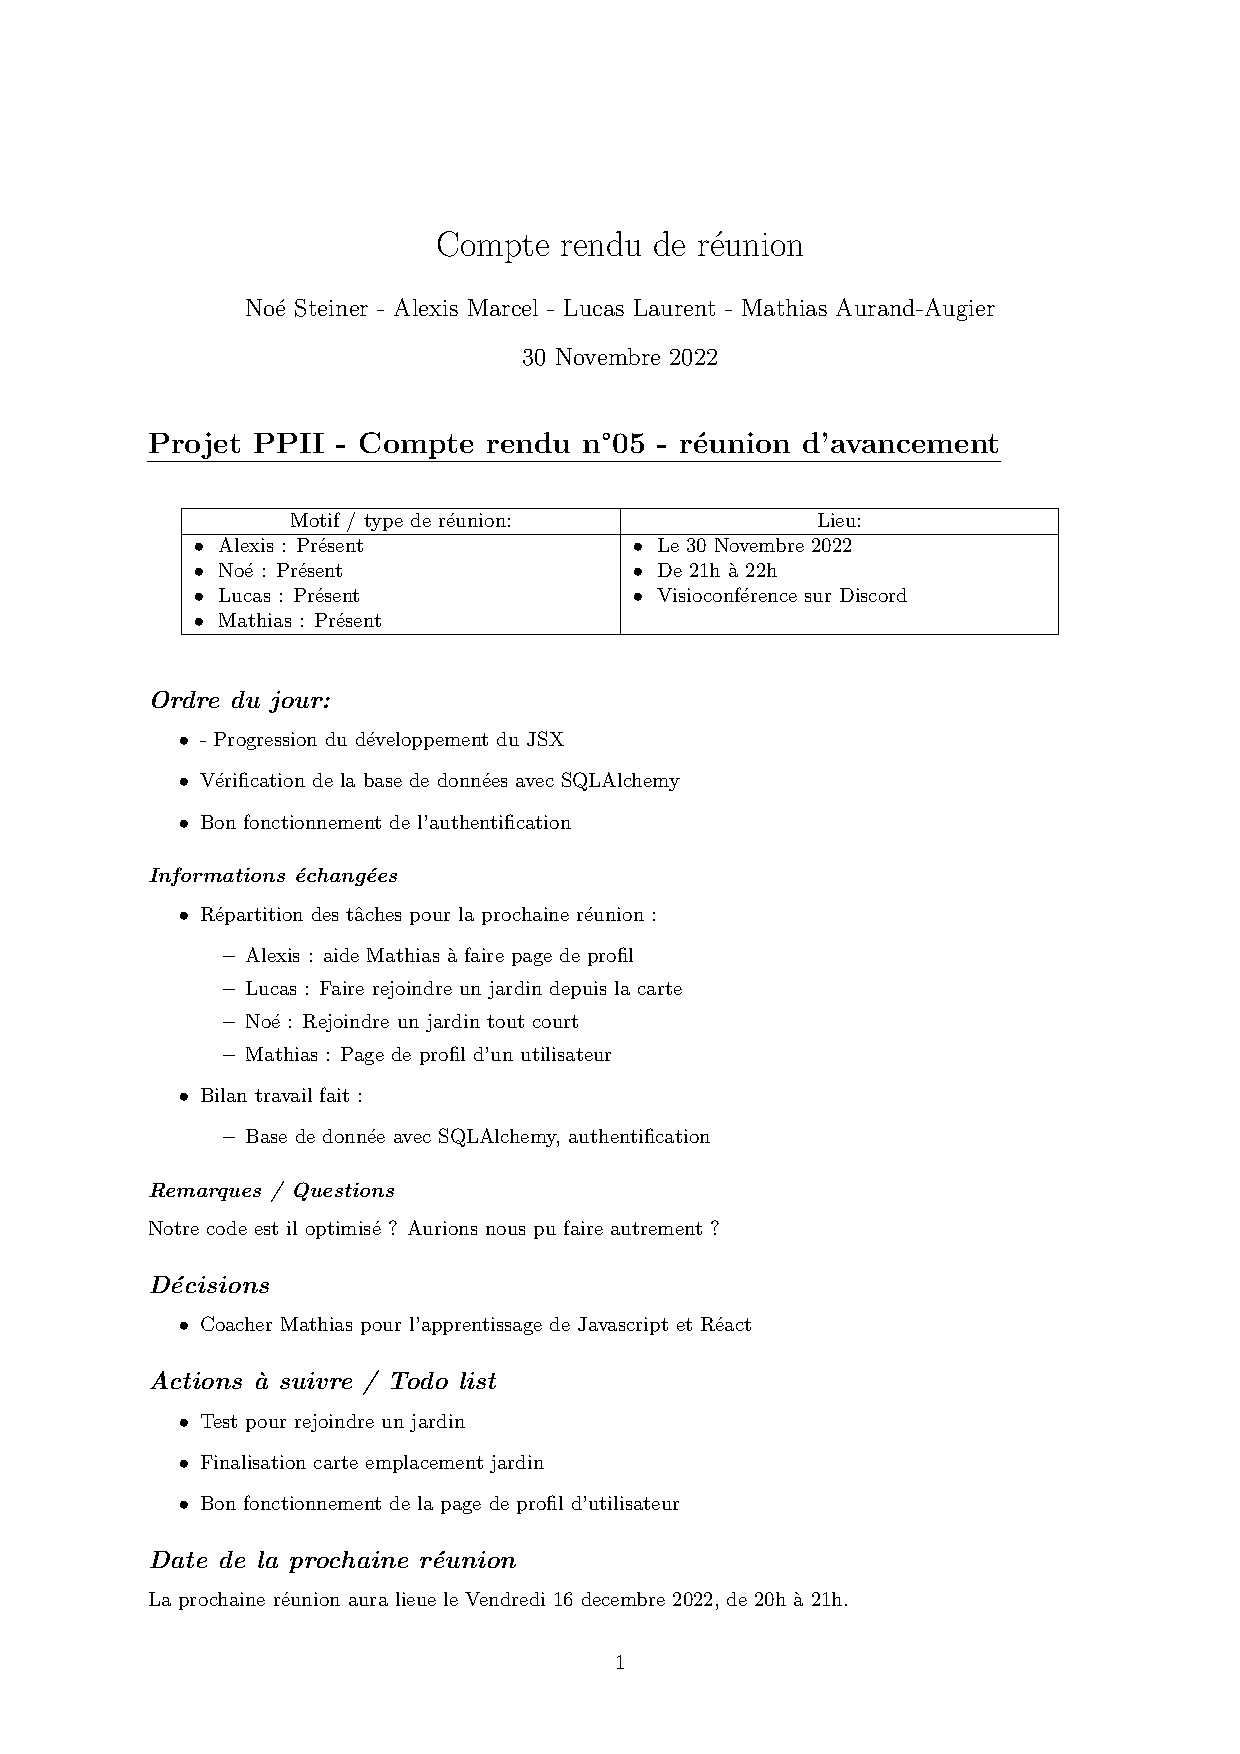
\includepdf[pages=1]{../../cr_reu/novembre/30/cr_30_novembre.pdf}
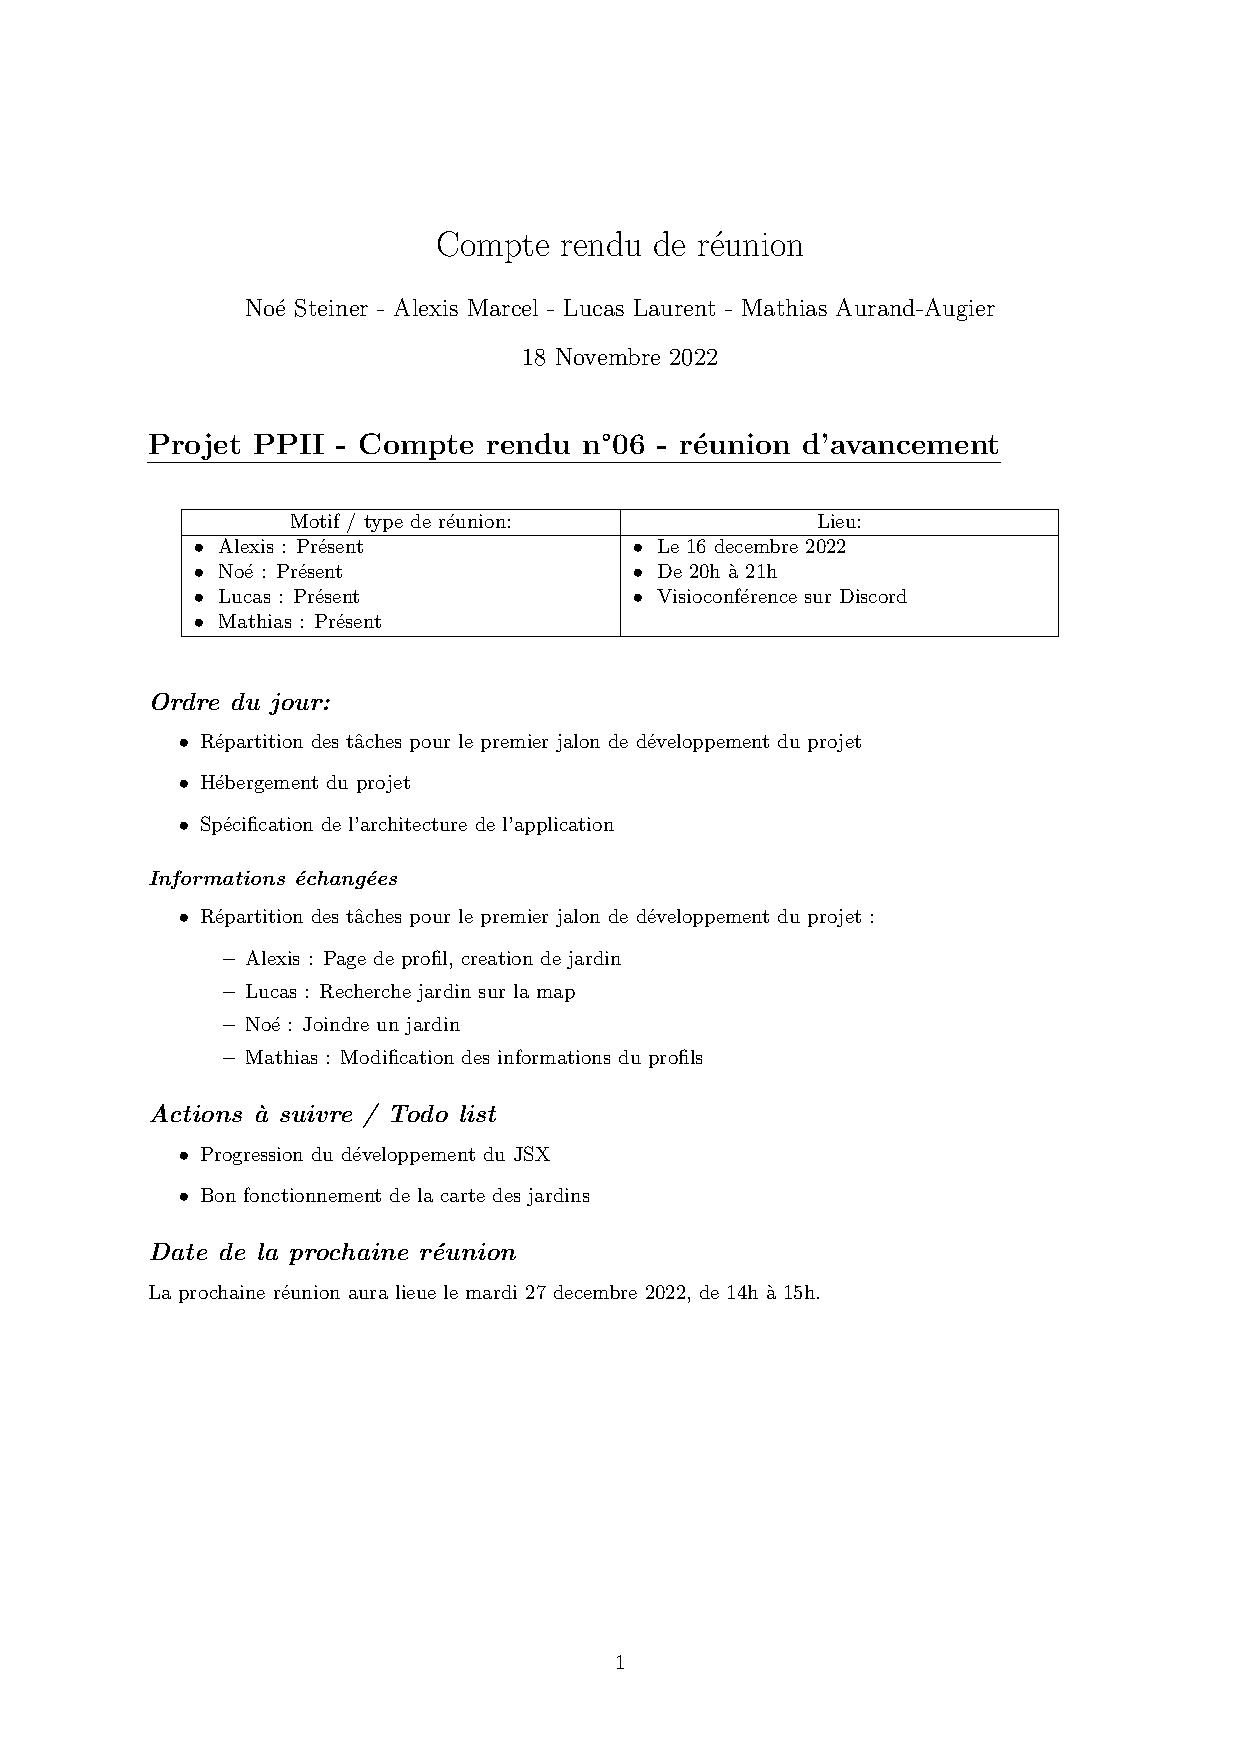
\includepdf[pages=1]{../../cr_reu/decembre/16/cr_16_decembre.pdf}
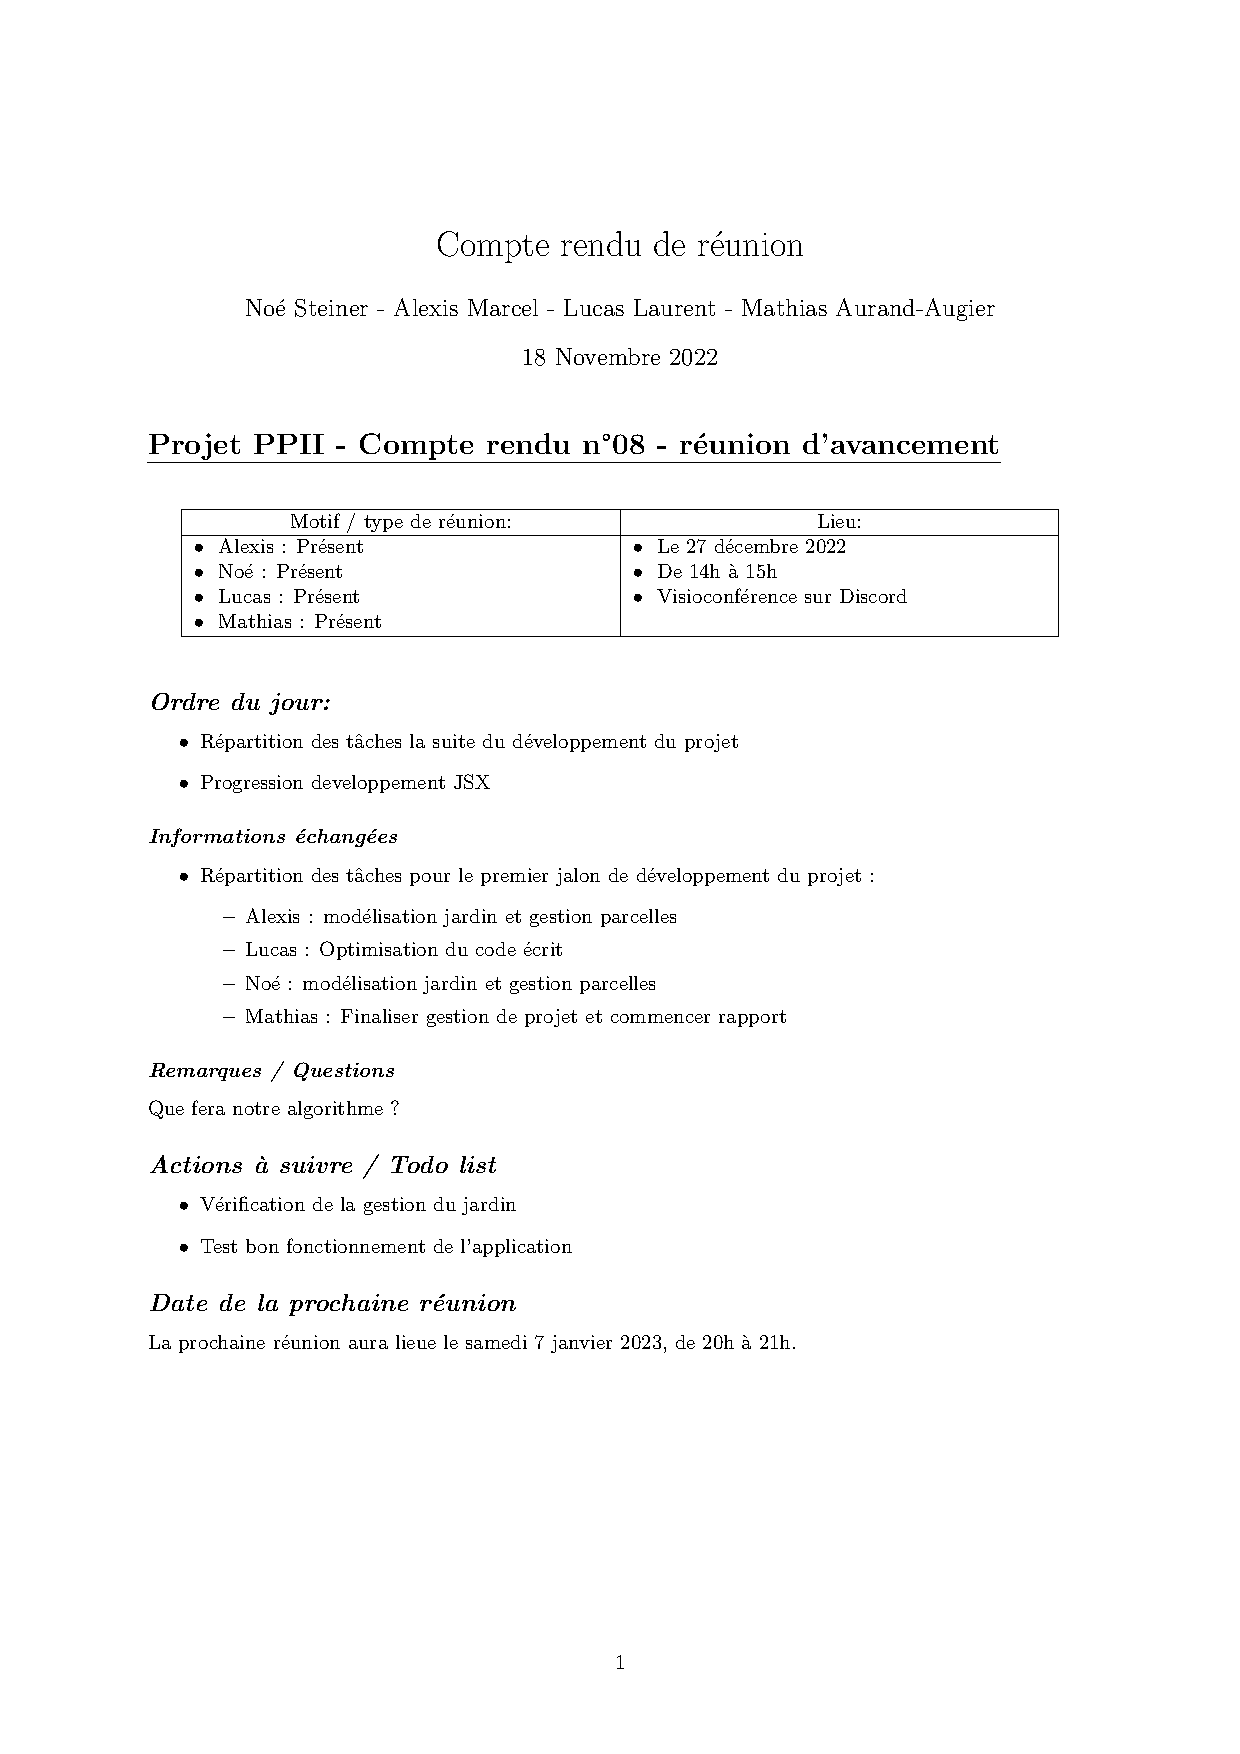
\includepdf[pages=1]{../../cr_reu/decembre/27/cr_27_decembre.pdf}
\end{document}